\documentclass{report}
\usepackage[pagestyles]{titlesec}
\usepackage[utf8]{inputenc}
\usepackage[margin=0.5in]{geometry}
\usepackage {graphics}
\usepackage{fancyhdr}
\usepackage{graphicx}
\usepackage{amsmath}
\usepackage{wrapfig}
\usepackage{float}
\usepackage{hyperref}
\usepackage{dirtytalk}
\usepackage{amsmath}
\usepackage{biblatex}
\usepackage{xcolor}
\usepackage{listings}
\usepackage{comment}
\usepackage[nottoc,numbib]{tocbibind}
\usepackage{algorithm}
\usepackage{algpseudocode}
\usepackage{tikz}
\usepackage{forest}
\usetikzlibrary{arrows.meta}
\usepackage{tikz-qtree}
\addbibresource{sample.bib}

\pagestyle{fancy}
\definecolor{codegreen}{rgb}{0,0.6,0}
\definecolor{codegray}{rgb}{0.5,0.5,0.5}
\definecolor{codepurple}{rgb}{0.58,0,0.82}
\definecolor{backcolour}{rgb}{0.95,0.95,0.92}
\lstdefinestyle{mystyle}{
    backgroundcolor=\color{backcolour},  
    commentstyle=\color{codegreen},
    keywordstyle=\color{magenta},
    numberstyle=\tiny\color{codegray},
    stringstyle=\color{codepurple},
    basicstyle=\ttfamily\footnotesize,
    breakatwhitespace=false,         
    breaklines=true,    
    frame=single,
    captionpos=b,                    
    keepspaces=true,                 
    numbers=left,                    
    numbersep=5pt,                  
    showspaces=false,                
    showstringspaces=false,
    showtabs=false,                  
    tabsize=2
}
\lstset{style=mystyle}

\hypersetup{
    colorlinks,
    citecolor=black,
    filecolor=black,
    linkcolor=black,
    urlcolor=black
}
%%%%%%%%%%%%%%%%%%%%%%%%%%%%%%%%%%%%%%%%%%%%%%%%%%%%%%%%%%%%%%%%%%%%
\setlength{\textwidth}{6.25in} % original 6.25
\setlength{\textheight}{8in}


\titleformat{\chapter}[display]{\normalfont\bfseries}{}{}{\Huge}

\newcommand\ytl[2]{
\parbox[b]{8em}{\hfill{\color{black}\bfseries\sffamily #1}~$\cdots\cdots$~}\makebox[0pt][c]{$\bullet$}\vrule\quad \parbox[c]{10.5cm}{\vspace{7pt}\color{red!40!black!80}\raggedright\sffamily #2.\\[0pt]}\\[-3pt]}
\renewcommand{\baselinestretch}{1.3}
\renewcommand{\contentsname}{Plan}
%\titleformat{\chapter}[display]{\normalfont\huge\bfseries\centering}
%\newcommand{\cchapter}[1]{\chapter[#1]{\centering #1}}

\oddsidemargin 20pt    %  Left margin on odd-numbered pages.
\evensidemargin 20pt   %  Note that \oddsidemargin = \evensidemargin
%\addtolength{\topmargin}{-.875in}
\topmargin 0pt
%%%%%%%%%%%%%%%%%%%%%%%%%%%%%%%%%%%%%%%%%%%%%%%%%%%%%%%%%%%%%%%%%%%%
%\usepackage{titlesec}

\begin{document}
%\usetikzlibrary{graphs,graphdrawing,arrows.meta}
%\usegdlibrary{trees}

\begin{titlepage}
\newpage
\pagestyle{empty}
\pagenumbering{gobble}
%\thisfancypage{cmds1}{cmds2}
%\thisfancyput(-0.0 in, -10.0 in) {\setlength{\unitlength}{1 in}\framebox(6.7,10.2)}
\vspace*{\fill}
\begin{center}
    \textbf{\huge Blockchain interoperability}\\
	\end{center}
\vspace*{\fill}    
\end{titlepage}

\newpage
\tableofcontents

\newpage
%%%%%%%%%%%%%%%%%%%%%%%%%%%%%%%%%%%%%%%%%%%%%
%\pagestyle{headings}
\pagenumbering{arabic}
\setcounter{page}{1}
\setcounter{tocdepth}{3}
\setcounter{secnumdepth}{3}

%%%%%%%%%%%%%%%%%%%%%%%%%%%%%%%%%%%%%%%%%%%%%
\begin{abstract}
   This post is intended to present the minimal understanding of how interoperability works and give a quick overview of some current solutions. For example, the details of the merkle trees in Ethereum are left in the appendix as it adds complexity and the post is hopefully understandable without it. \\
   We first present the background needed in blockchain with a focus on merkle trees as they are mainly used in interoperability solutions. 
   \\ We then define interoperability and explain how some interesting protocols are achieving it.
\end{abstract}
\chapter{Background}
\section{Merkle tree}
Ralph Merkle invented the merkle trees in 1979. We present here the binary merkle tree used in bitcoin and a derivation of the patricia merkle tree used in ethereum.
\subsection{Binary merkle tree}
\begin{figure}[H]
    \centering
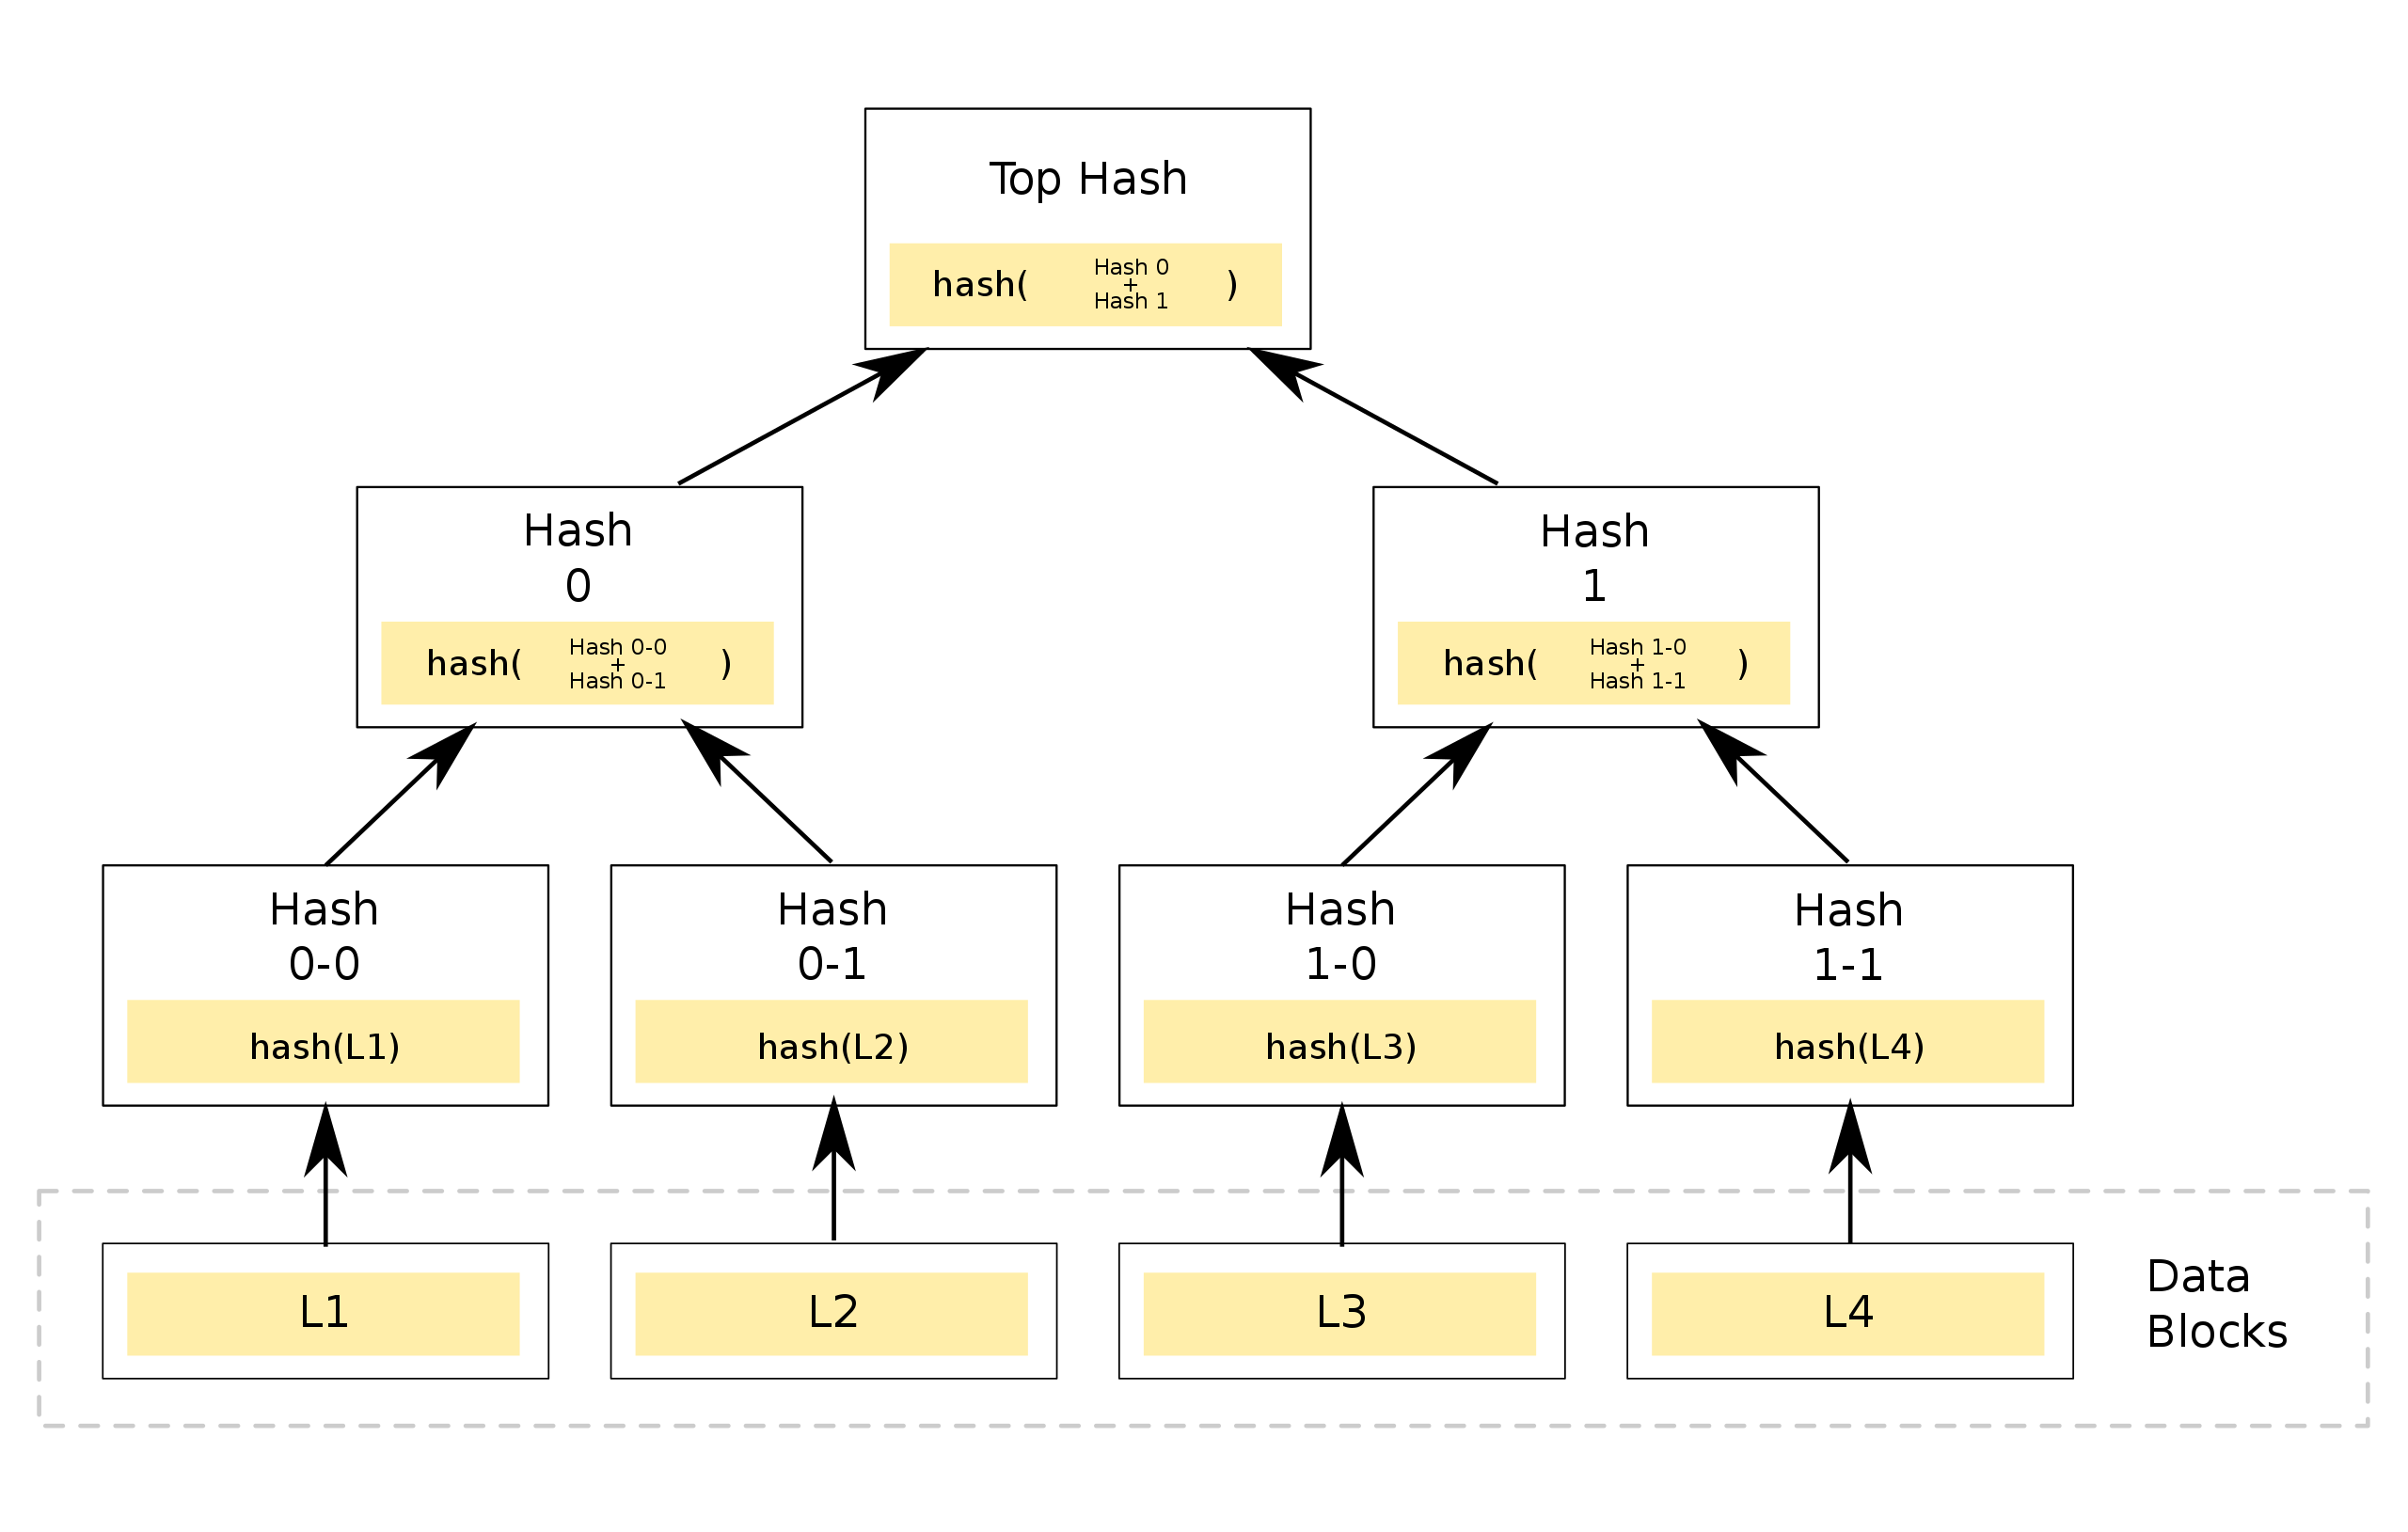
\includegraphics[width=0.7\linewidth]{background/merkle.png}
    \caption{Binary merkle tree}
    \label{fig:merkle}
\end{figure}
The binary merkle tree consists of hashing the transaction two by two: 
\begin{enumerate}
    \item List all the data you want to save in an ordered list: it can be n users for example or any kind of data. In blockchain, these data are the transactions. Here say we have 4 transactions L1, L2, L3, L4.
    \item Hash these data one by one to obtain n hashes. Here we obtain 4 transactions hashes \\($Hash_{0-0},Hash_{0-1},Hash_{1-0},Hash_{1-1})$
    \item Hash the hashes two by two starting from the left. If there is only one node on the right of the tree, we duplicate it two obtain the parent. Here we obtain $Hash_0, Hash_1$.
    \item Repeat the last step until we obtain only one node left: the root.
\end{enumerate}
The root is a fingerprint of all the data, in our case the four transactions. 
It means that if you change anything in the original data, the timestamp of the first transaction for example, it'll change completely the root hash of the merkle tree, thanks to the non locality property of the hash function used (Alice and Aline have very different hashes even if they have only one different letter)

\subsection{Proof of inclusion} \label{merkle:inclusion}
Merkle trees allow to summarize the data into one fixed length fingerprint, the root hash. 
But why should we use this data structure instead of just hashing all the hashes for example?

This data structure allows proof of inclusion. In the case of bitcoin for example, data is the transactions, and this structure allows other users to answer this question: \\
\textbf{Is this transaction really included in that block?}

So let's consider the merkle tree below:

\begin{figure}[H]
  \centering
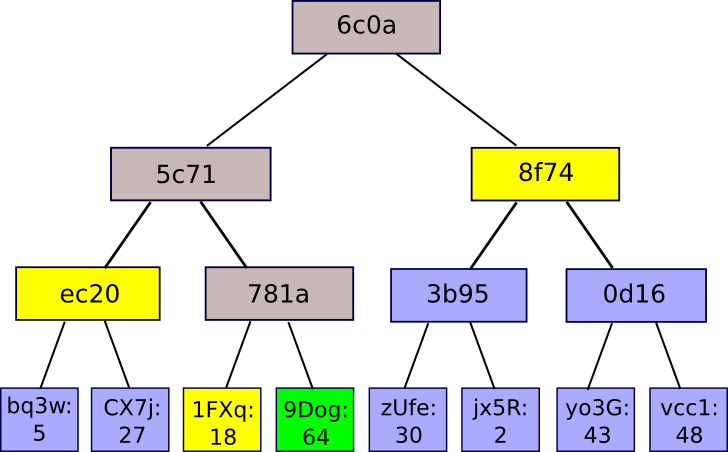
\includegraphics[width=0.5\linewidth]{background/merkle_proofs_2.png}
\caption{Proof of inclusion in merkle tree}
\end{figure}

We have 8 transaction hashes that we want to place in the merkle tree in this example. Let's say we are interested in the transaction in green (9Dog:64) because it's directed to our account. We want a proof that this transaction has really happened, and have been included in that block with merkle root 6c0a. 

The proof is a merkle block with the yellow hashes. The verifier of this proof can then follow these steps:
\begin{enumerate}
    \item With green transaction and the yellow one 1FXQ:18 you can concatenate and hash it to get the parent hash 781a.
    \item With this last hash 781a and the yellow one ec20 you can concatenate and hash them to get the parent hash 5c71.
    \item And with this last hash concatened with the last yellow one 7f74 and hashed, we get the merkle root
    \item We compare the calculated merkle root from the proof and the real one from the block. If they match, the proof is accepted.
    In bitcoin, it means that the transaction is included in this block. If they don't , we cannot prove the inclusion with that proof. 
\end{enumerate} 

\textbf{
What is the advantage of using this data structure?}

The verifier only needs the merkle root of the block to accept the proof of inclusion. But as this is a binary tree, the number of hashes at each level is divided by two, so this proof only consists of $\log_2(n)$ hashes, with n the number of transactions. 
It means that if we have 8 transactions, as in this example we  need one hash per level so $\log_2(8)=3$ hashes to proof the inclusion of the transaction in the block.

\colorbox{lime}{
\textbf{
If $n=100$ we need $\log_2(100)\sim 7$ hashes, if $n=1000$ we need $\log_2(1000)\sim 10$ hashes.
}
}


\section{Blockchain basics}

The blockchain can be viewed as a replicated state machine. It means that  each time $t$ is associated with a global state which goes to the next state at $t+1$ with the state transition function. 

Here the state is for example account balances for bitcoin, the state transition function represented by the transactions, instructions to be executed to go to the next state.
In blockchain, the transactions for each state transition are placed in a new block, adding to the chain of blocks.
\begin{figure}[H]
\centering
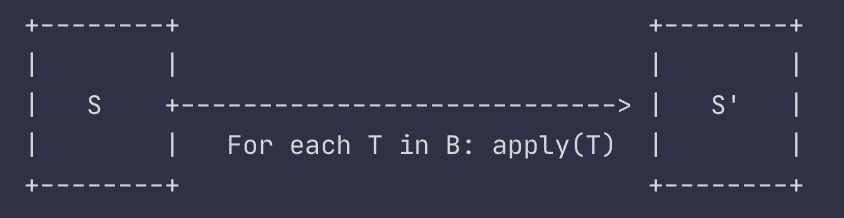
\includegraphics[width=0.6\linewidth]{background/state_transition.png}
    \caption{The state S transitioning to state S' by executing all transactions T from the block B}
    \label{fig:state_transition}
\end{figure}
Lastly, it is replicated across all the full nodes to ensure global consistency of the distributed ledger, meaning that the nodes on the network should agree on the blockchain state thanks to the consensus algorithm.

\subsection{The block}
So what is stored exactly in a block? 

Let's say for the moment that the bitcoin block consists of:
\begin{itemize}
    \item the hash of the previous block. You take the whole previous block and pass it to the hash function.
    \item the nonce resulting from the cryptographic puzzle. We'll talk about it later. 
    \item the list of transactions included in the block.
\end{itemize}
\begin{figure}[H]
    \centering
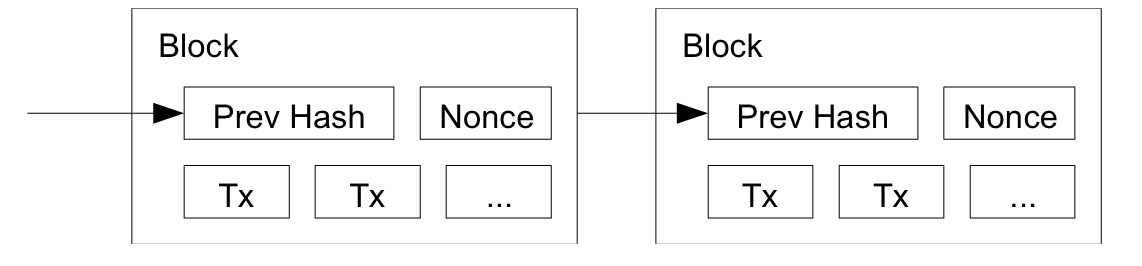
\includegraphics[width=0.6\linewidth]{background/block.png}
    \caption{A bitcoin block: the hash of the previous block, the nonce, and the list of transactions}
    \label{fig:block}
\end{figure}

This requires every node in the network to keep the list of transactions since 2009.

\subsection{Merkle tree of transactions}
In fact, the block is composed of the block header and the list of transactions. The block header contains this time the root hash of the transactions merkle tree.
The root hash is a summary of all the transactions happening during that period represented a merkle tree. For bitcoin, binary merkle tree are used for transactions, whereas in Ethereum, merkle Patricia trees are used to store transactions, state, receipts. 
\begin{figure}[H]
    \centering
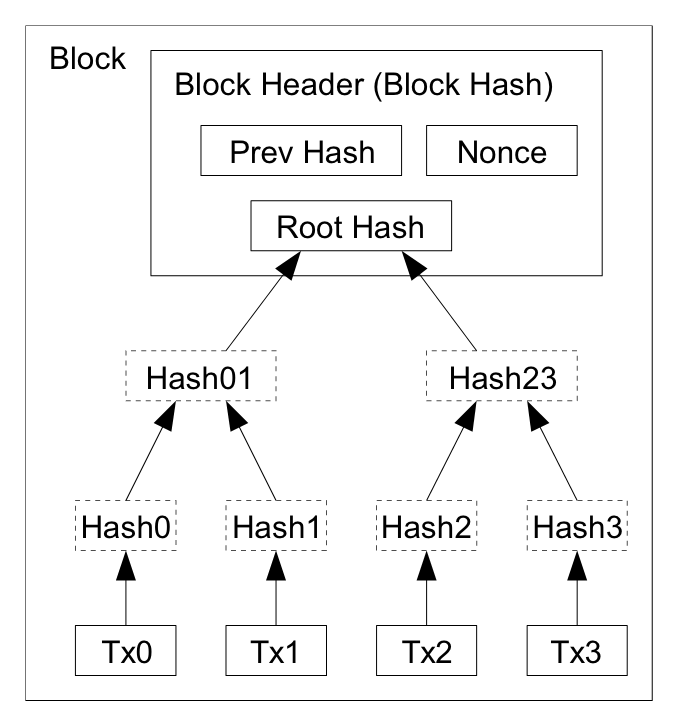
\includegraphics[width=0.4\linewidth]{background/blockmerkle.png}
    \caption{A Bitcoin\cite{Nakamoto..09} block}
    \label{fig:blockmerkle}
\end{figure}

\subsection{Single payment verification}
This allows two actors to emerge: \\
\textbf{The full node} stores all the full blocks, with the transactions. With this transactions, it can provide the proof of inclusion: the hashes required to prove a transaction is in a particular block. \\
\textbf{The light node } asks for the blocks headers to the full nodes of the network. Once he got the block headers, he can ask the full nodes of the network to provide a proof for the transactions is interested into. With the procedure described in \ref{merkle:inclusion}, the light node can verify that the transaction has indeed happened in the blockchain.

The light node is only storing the block headers, so even a phone can handle the amount of storage needed. This allows for example to verify with your wallet that a transaction has been executed  on your laptop without downloading the $\sim 500$GB of the blockchain.



\chapter{Interoperability}
Merkle proofs from \ref{merkle:inclusion} are used to prove to a light client that a transaction has happened. \\
\textbf{Now this can be used to prove to blockchain B that a transaction like a token transfer has taken place in a blockchain A.}

In this chapter let's see how interoperability between blockchains can be achieved using merkle proofs. 

\section{Interoperability with merkle proofs}

\section{Examples}
So, now that we understand the merkle proofs, \textbf{how are they used in current interoperability solutions?}
\\We present a rapid overview of some interesting solutions, the goal here is to understand where the merkle proofs step in and how they help achieving interoperability in these protocols, leaving many details uncovered to keep it simple.
\subsection{LayerZero \cite{zarick2021layerzero}}
\begin{figure}[H]
    \centering
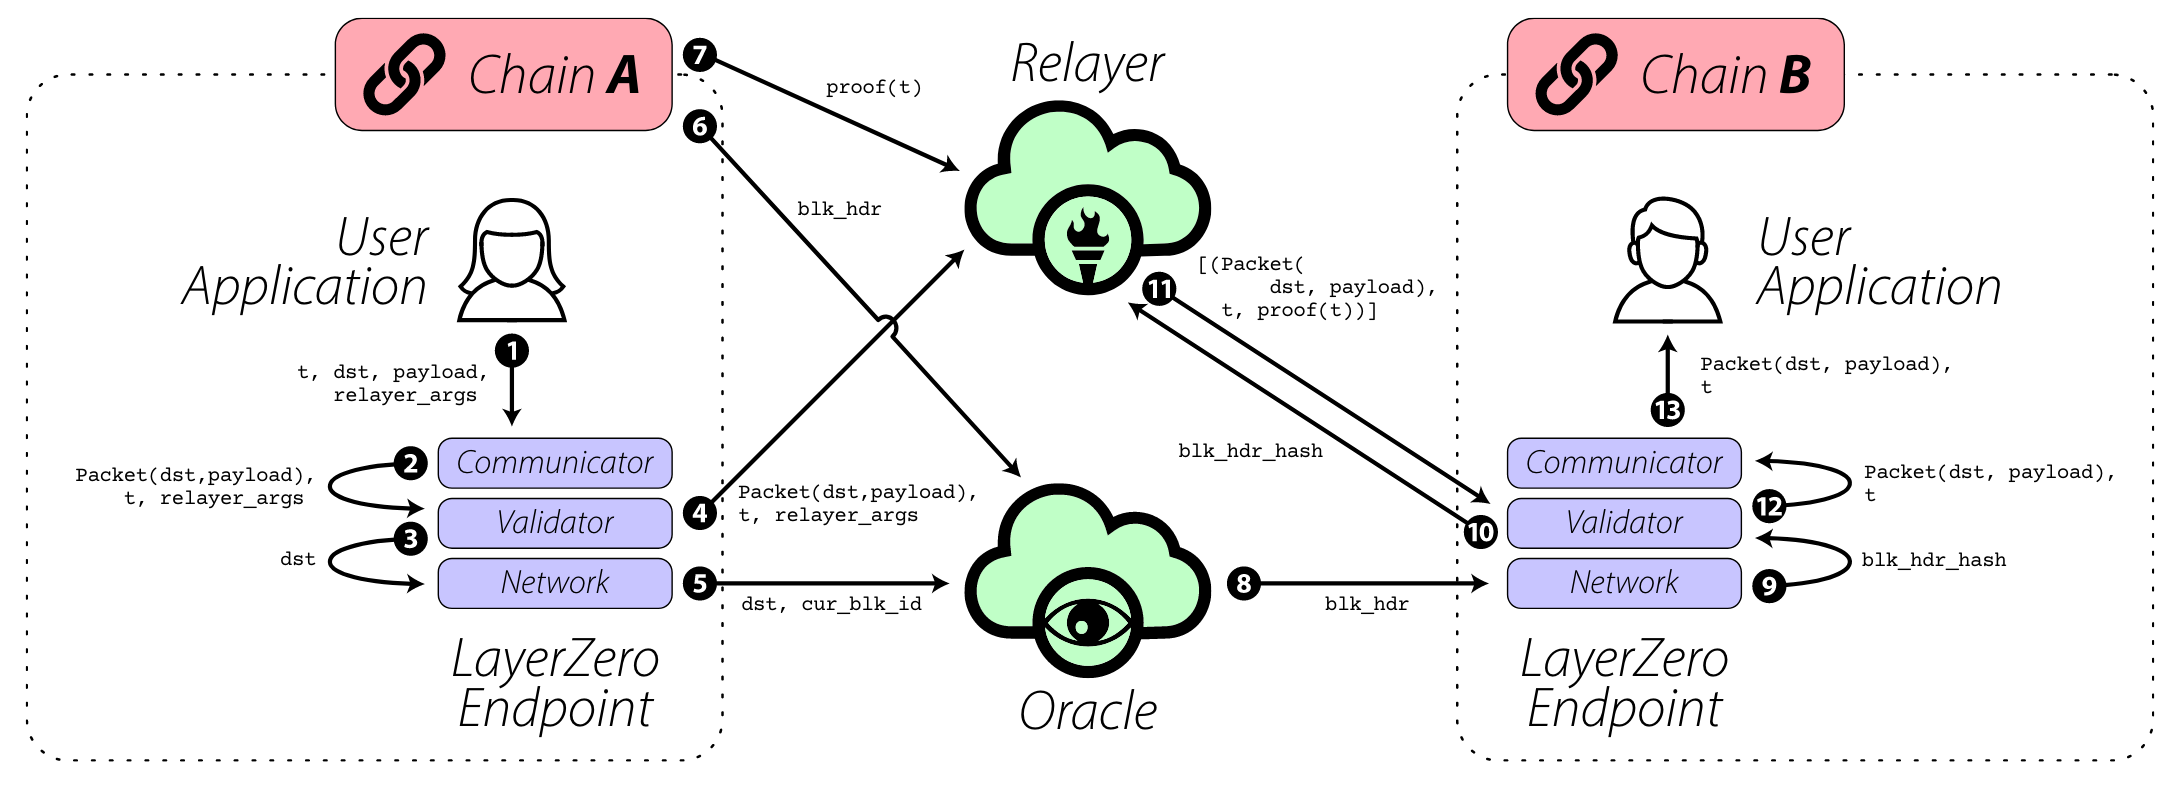
\includegraphics[width=1.\linewidth]{interoperability/layerZero.png}
    \caption{LayerZero}
    \label{fig:layer_zero}
\end{figure}

For each supported chain, LayerZero deploys an endpoint, consisting in 4 smart contracts. This endpoint includes a library handling the verification of the transaction proof.

So, from \ref{merkle:inclusion},  to verify that a transaction has taken place we need the merkle root, included in the block header and the the merkle proof. 
\\
LayerZero offers interoperability by transporting these two necessary pieces of data.
\begin{itemize}
    \item The block header containing the merkle root is carried by the oracle from blockchain A to blockchain B. 
    \item The merkle proof of blockchain A is carried by a relayer from blockchain A to blockchain B.
\end{itemize}

The oracle is a Chainlink oracle monitoring the source blockchain and the relayer can be handled by LayerZero or anyone interested into this. 
\\
Chain B can then attest that the transaction has happened by verifying the proof against the block header sent by the oracle.

\textbf{The security of LayerZero relies on the independence of the relayer and the oracle.}

If the oracle and the relayer collude, they can give a fake block header, and a proof working with that fake block. 


\subsection{ZKBridge \cite{xie2022zkbridge}}
\begin{figure}[H]
    \centering
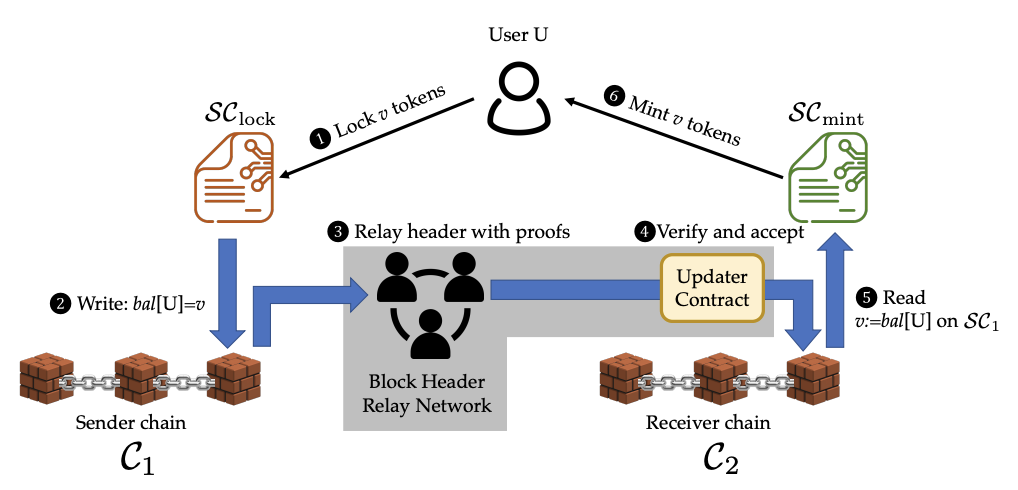
\includegraphics[width=0.8\linewidth]{interoperability/zkbridge.png}
    \caption{ZKbridge}
    \label{fig:zkbridge}
\end{figure}

Zero knowledge proofs are introduced here: \ref{zeroknowledge}.

So here, the gray part is ZKbridge.
\\The most important part is done here by the relayers. 
\begin{enumerate}
    \item The relayers contact the full nodes of blockchain C1 to get the last block header% $blkH_r$ following the $blkH_{r-1}$
    \item the relayers generate a zero knowledge proof that a light client of the sender chain C1 accepts that block header
    \item This proof is then sent to the ZKBridge updater contract of the receiving chain C2
    \item this updater contract verifies the ZK proof and adds it to its list of block headers if successfully verified.
    \item The application contract, anyone on C2 can call the public function GetHeader from the updater contract to get the header. 
\end{enumerate}

Zk bridge achieve interoperability by verifying the validity of the block header. The relayers do that in a indirect way : they prove by a zk proof that a light client of the source chain accepts this block header. 
\\
Let's understand what the acceptance of the light client means. 
In ethereum, it means that: 
\begin{itemize}
    \item the status of the block header is finalized. Finality means that you can be sure it'll not be reverted. 
    \item the sync committee, group of validators, have sufficient participants 
    \item the aggregated signature is correct, meaning that the aggregator in Ethereum received enough votes and signed it.
\end{itemize}


\textbf{The security of the ZKbridge relies notably on the security of the light client of C1.} It's because the zero knowledge proof consists in proving that this light client accepts the block.
\subsection{Telepathy}

\begin{figure}[H]
    \centering
    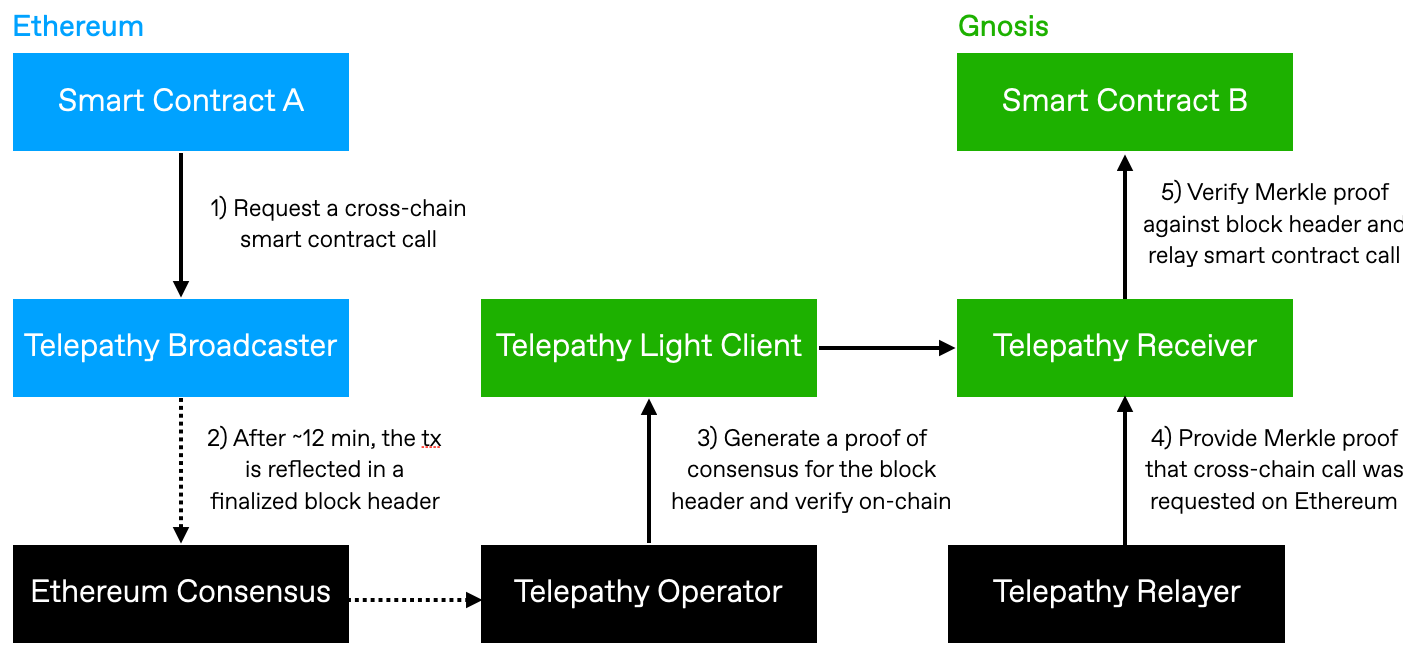
\includegraphics[width=0.8\linewidth]{interoperability/telepathy.png}
    \caption{Telepathy workflow}
    \label{fig:telepathy}
\end{figure}

Telepathy is based on proof of consensus. It means that to prove that a block header from blockchain A is valid, it will basically check that a large majority of the validators signed the block header. But verifying all these signatures one by one is computationally expensive. Instead the proof used in Telepathy is a zero knowledge proof attesting that the block header has been signed by a sufficient percentage of validators. 

The zero knowledge proof can be cheaply verified onchain and chain B can then expose these verified blockheaders.
The smart contract in chain B can then verify the merkle proof relayed by the Telepathy relayer against the verified block header 

\textbf{The security of the Telepathy relies directly on the honesty of the Ethereum validator set (sync committee validators).
}


\newpage
\printbibliography[title={Références}]
\newpage
\appendix
\chapter{Appendix}
This part is placed in the appendix because it adds complexity and is not absolutely necessary to understand the main ideas on the interoperability. 

\section{Merkle trees}
\subsection{Trie}
Binary merkle tree are used in bitcoin. 
In Ethereum a more complicated version is used, derived from the patricia trie. First let's understand what a trie is. 
\begin{figure}[H]
    \centering
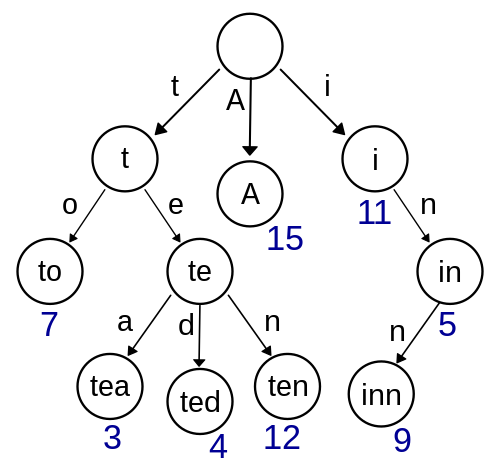
\includegraphics[width=0.3\linewidth]{background/trie.png}
    \caption{Trie representing the words "A", "to", "tea", "ted", "ten", "i", "in", and "inn"}
    \label{fig:trie}
\end{figure}
A trie is a tree data structure where the key of the node is also his path from the root. The key is usually a string.
In other words positions in the trie is determined directly from the key and the inverse is correct. 

Let's say you want to save n words in the trie:
\begin{enumerate}
    \item From the root, at step 1 we take the first letter of each of the n words and create a leaf for each different ones. In the example from the figure above, we  take A from A, t from to, tea, ted, ten, i from i, in and inn. We have then 3 nodes from the root: t, A, i
    \item at step t, repeat the first step but instead take the t first letters. 
    \item stop when all the original words are in a leaf. 
\end{enumerate}
If we have a string with 200 letters, we'll have to create 200 levels.
\subsection{Patricia trie}
As said in the last section, if you have a n length word you'll have to create n levels, which is not optimized in term of storage. 
Instead, radix tree and Patricia tree are a compressed version of the above trie.
\begin{figure}[H]
    \centering
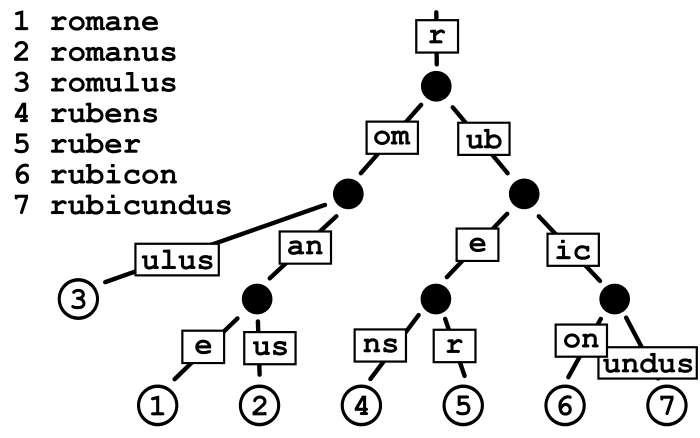
\includegraphics[width=0.4\linewidth]{background/patricia.png}
    \caption{Patricia tree}
    \label{fig:patricia}
\end{figure}
Here, we are not limited at each step in terms of length of the key.

\subsection{Patricia merkle tree}

\begin{figure}[H]
    \centering
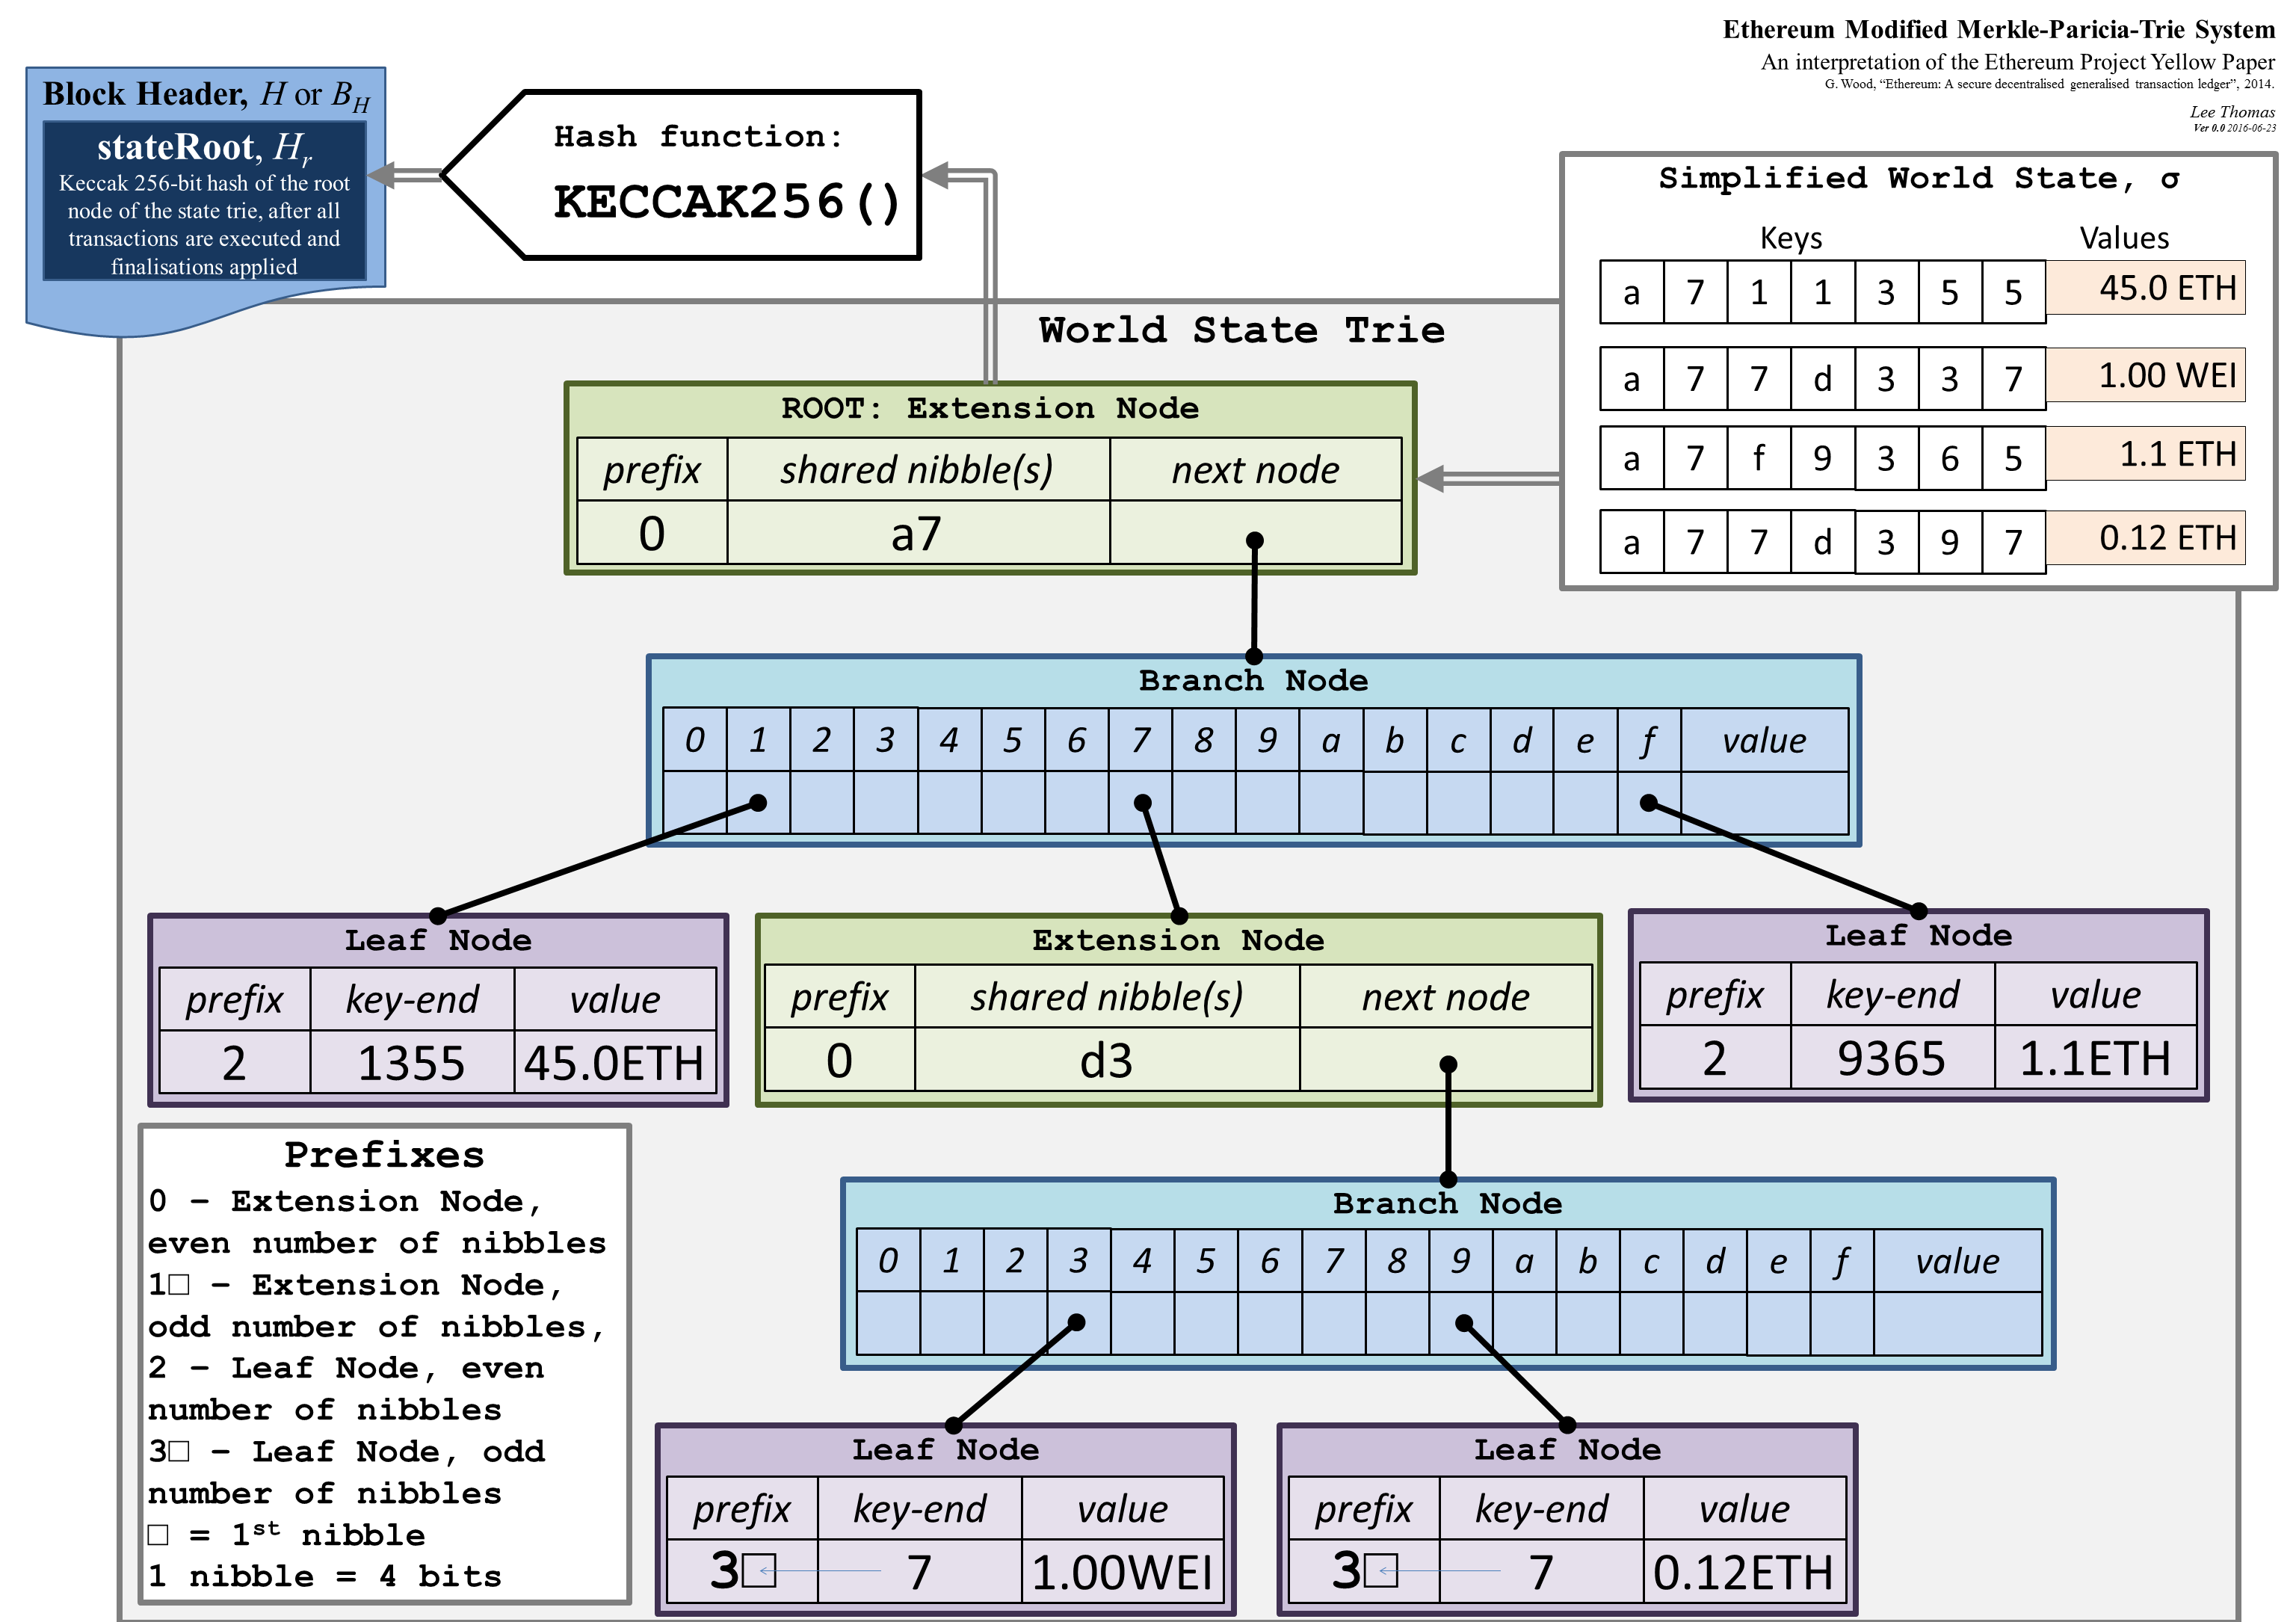
\includegraphics[width=0.9\linewidth]{background/ethereum_mpt.png}
    \caption{Ethereum patricia tree}
    \label{fig:eth_mpt}
\end{figure}

The Patricia merkle tree used in Ethereum modifies the original Patricia tree. The keys are hexadecimal strings and defines 4 types of nodes: 
\begin{itemize}
    \item EmptyNode represented as the empty string
    \item BranchNode: a 17-item node [ v0 ... v15, vt ]
    \item LeafNode: a 2-item node [ encodedPath, value ]
    \item ExtensionNode: a 2-item node [ encodedPath, key ]
\end{itemize}
A branch node at a certain step t, at letter t, is created when there are multiple possible letters for the next letter at $t+1$. Since we use hexadecimal keys, at each step we can choose between 16 letters (or the value).

A leaf node is the last possible node in the branch and contains the value. Here we can say that the key represents the adress of the ethereum account and the value is the balance. 

The extension node is the compression offered by the Patricia trie. It represents the shared nibbles (letter) before two or more words diverge. 



Ethereum\cite{Buterin..13} stores three merkle roots in the block header. One for the transactions as in bitcoin, another one for the state (balances for example), and another one for the receipts. 

\colorbox{lime}{
These merkle trees allows Ethereum to answer more questions than just the inclusion of a transaction.
}
\begin{itemize}
\item Has this transaction been included in a particular block?
\item Tell me all instances of an event of type X (eg. a crowdfunding contract reaching its goal) emitted by this address in the past 30 days
\item What is the current balance of my account?
\item Does this account exist?
\item Pretend to run this transaction on this contract. What would the output be?
\end{itemize}


\section{Zero knowledge}
\label{zeroknowledge}
This is meant to be a light introduction to the zero knowledge proof concept to understand the following interoperability solutions. 

A zero-knowledge protocol is a method by which one party (the prover) can prove to another party (the verifier) that something is true, without revealing any information apart from the fact that this specific statement is true. \cite{Goldwasser}

For example, in digital signature, you send a signature proving that you are indeed the one sending the mail. More precisely, this signature prove that you know the private key without revealing it. The verifier checks that the signature matches the public key of the sender. ( $\sim$ signature reveals the public key)
\\Instead of only proving that you know the private key as in digital signatures, zero knowledge proofs can prove "any type" of computation. 
\\For example, you can prove that: 
\begin{itemize}
    \item you know m when you send H=SHA3(m) to the verifier, without revealing m. 
    \item you know a sudoku solution to a sudoku problem without revealing it 
    \item you know the $1000^{th}$ fibonacci number ( $a_{n-2}+a_{n-1}=a_n$)
    \item the transactions are valid. This allow the ZK roll-ups to process the transactions off chain, and prove on chain to layer 1 that these transactions are indeed valid. 
\end{itemize}

In fact, zero knowledge proofs allow two properties. 

\textbf{Computational integrity} prove that you have done the right computation, even when no one is watching. For example, in ZK-rollups the computational integrity is the main need and the privacy is not always/often taken into account. 

\textbf{Privacy} with zero knowledge, you don't reveal anything about the statement. In Zerocash\cite{sasson2014zerocash}, the privacy is needed to ensure the confidentiality of the transactions. 


\paragraph{} A zero knowledge protocol should verify:
\begin{itemize}
    \item \textbf{Completeness}: If the claim is valid, the verifier accepts the proof.
\item \textbf{Soundness}: If the claim is invalid, the verifier should reject the proof with very high probability.

\item \textbf{Zero-knowledge}: The verifier learns nothing about a statement beyond its validity or falsity 
\end{itemize}

To conclude, some important properties are expected from these protocols. We want of short proof in terms of size for example. We also want, and this is a fundamental requirement, a very fast verification. If the prover with a highly efficient computer computes the hash of a 200GB document, the verification should be very fast and consists in a much lighter computation than the prover one.

This last requirement is at the heart of the zero knowledge research and explains the complexity of the techniques used.

\end{document}
